\documentclass[11pt,a4paper]{article}

% --- Core Packages ---
\usepackage[utf8]{inputenc}
\usepackage[T1]{fontenc}
\usepackage[margin=1in,bottom=1.2in]{geometry}
\usepackage{helvet}
\renewcommand{\familydefault}{\sfdefault}
\usepackage{xcolor}
\usepackage{graphicx}
\usepackage{fancyhdr}
\usepackage{titlesec}
\usepackage{hyperref}
\usepackage{tcolorbox}
\usepackage{booktabs}
\usepackage{lastpage}
\usepackage{tikz}
\usetikzlibrary{shadows,calc}

% --- Modern Color Palette ---
\definecolor{primaryGold}{HTML}{D4AF37}
\definecolor{deepBlack}{HTML}{0A0A0A}
\definecolor{lightGray}{HTML}{F5F5F5}
\definecolor{accentBlue}{HTML}{0052FF}

% --- Header and Footer Styling ---
\pagestyle{fancy}
\fancyhf{}
\renewcommand{\headrulewidth}{0.4pt}
\renewcommand{\headrule}{\hbox to\headwidth{\color{primaryGold}\leaders\hrule height \headrulewidth\hfill}}

\fancyhead[L]{\textcolor{deepBlack}{\textbf{BotIn System Architecture}}}
\fancyhead[R]{\textcolor{primaryGold}{\textit{Protocol Infrastructure}}}

\fancyfoot[L]{
    \begin{tikzpicture}[remember picture,overlay]
        \node [anchor=south west, xshift=1in, yshift=0.5cm] at (current page.south west) {
            \begin{minipage}{\textwidth}
                \scriptsize
                \textcolor{gray}{2026 \textbf{c0bw3b Inc.} All Rights Reserved. | \\
                Llakterian @ c0bw3b Inc.}
            \end{minipage}
        };
    \end{tikzpicture}
}
\fancyfoot[R]{\textcolor{gray}{\thepage\ / \pageref{LastPage}}}

% --- Section Styling ---
\titleformat{\section}
  {\color{deepBlack}\normalfont\Large\bfseries}
  {\thesection}{1em}{}[{\titlerule[0.8pt]\vspace{2pt}\color{primaryGold}\titlerule[1.5pt]}]

\titleformat{\subsection}
  {\color{deepBlack}\normalfont\large\bfseries}
  {\thesubsection}{1em}{}

% --- Custom Boxes ---
\newtcolorbox{premiumbox}[1]{
  colback=lightGray,
  colframe=primaryGold,
  fonttitle=\bfseries,
  title=#1,
  enhanced,
  drop shadow,
  sharp corners=southwest
}

\begin{document}

\begin{center}
    \vspace*{1.5cm}
    {\Huge \textbf{\textcolor{deepBlack}{System Architecture}}} \\
    \vspace{0.5cm}
    {\Large \textcolor{primaryGold}{BotIn Protocol Blueprint}} \\
    \vspace{1.5cm}
    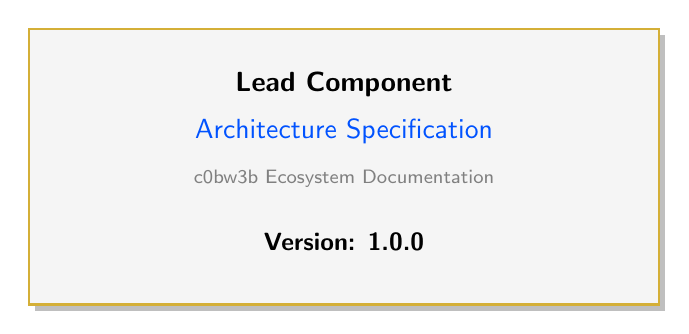
\begin{tikzpicture}
        \draw[fill=lightGray, draw=primaryGold, line width=1pt, drop shadow] (0,0) rectangle (8,3.5);
        \node at (4,2.8) {\textbf{Lead Component}};
        \node at (4,2.2) {\textcolor{accentBlue}{Architecture Specification}};
        \node at (4,1.6) {\scriptsize \textcolor{gray}{c0bw3b Ecosystem Documentation}};
        \node at (4,0.8) {\small \textbf{Version: 1.0.0}};
    \end{tikzpicture}
    \vspace{1.5cm}
\end{center}

\section{Core Architecture}
BotIn implements a highly modular, event-driven architecture designed for extreme scalability and trustless execution on the Base (Ethereum L2) ecosystem.

\subsection{Key Pillars}
\begin{itemize}
    \item \textbf{Low-Latency Identity:} Powered by Base Sepolia/Mainnet.
    \item \textbf{Standardized Agents:} Native compliance with ERC-8004.
    \item \textbf{Abstracted Transactions:} Seamless onboarding via ERC-4337 (AA).
    \item \textbf{Sovereign Messaging:} Distributed encryption powered by XMTP (v3).
    \item \textbf{Economic Stability:} All protocol settlement occurs in USDT.
\end{itemize}

\section{Protocol Layers}

\subsection{1. Identity Registry (ERC-8004)}
The authoritative source of truth for agent identities. Mints ERC-721 NFTs that serve as sovereign identifiers.

\subsection{2. Payment Vault (Settlement)}
Handles all pecuniary interactions within the ecosystem, managing economic gates for agent verification levels.

\subsection{3. Reputation Registry}
The trust layer of the network, enabling auditable peer-to-peer validation through immutable logs.

\section{Strategic Roadmap}
\begin{enumerate}
    \item \textbf{Treasury Hardening:} Formal transition to Gnosis Safe (Multisig).
    \item \textbf{L2 Expansion:} Cross-chain identity synchronization.
    \item \textbf{Particle Integration:} Social Login to Embedded Smart Account transition.
    \item \textbf{AI Verification:} Automated TEE (Trusted Execution Environment) attestations.
\end{enumerate}

\end{document}
